%% Los margenes, tipo de hoja y estilo BOOK
\documentclass[a4paper,11pt,twoside,openright,titlepage]{book}
\usepackage[a4paper,left=1in,right=1in,top=0.6in]{geometry}

\usepackage[T1]{fontenc}    %Intérprete de tildes
\usepackage[utf8]{inputenc}

\usepackage{amsmath,amssymb}    %Paquete de entornos matematicos

\usepackage{natbib}
\usepackage[english,spanish]{babel}
\selectlanguage{spanish} 
\usepackage{graphicx}
\usepackage{psfrag}
\usepackage{quotchap}
\usepackage{epsfig}
\usepackage[all]{xy}

\usepackage{epsfig}
\usepackage{makeidx}
\usepackage{ifthen}
\usepackage{multicolpar}    %Para poner texto en columnas en plan articulo intercalado con texto normal
\usepackage{multicol,multirow}

\usepackage{url}        %Para direcciones web
\usepackage{marvosym}   %Para imprimir el simbolo de \EUR euro
%\usepackage{eurosym}   %Para imprimir el simbolo de \euro euro
\usepackage{fancybox}   %Para tablas con bordes redondeados


%% Modificación de la plantilla para adaptarla a los requisitos de PFC
\usepackage{fancyhdr}
\pagestyle{fancy}
%%% Cabeceras y pies de página
\fancyhead[CE,CO]{\emph{\titulo}}
\fancyhead[LE,LO,RE,RO]{}
\fancyfoot[LE,RO]{\thepage}
\fancyfoot[CE,CO]{\leftmark}

\renewcommand{\footrulewidth}{.6pt}


%Definiciones de funciones para los títulos
\newlength\salto
\setlength{\salto}{3.5ex plus 1ex minus .2ex}

\newlength\resalto
\setlength{\resalto}{2.3ex plus.2ex}

\newcommand{\lsection}[1]
                {\section{#1}
                \vskip-.9\resalto   %%%% Aquí reculo el posible salto por defecto de \section
                \hrule
                \vskip+.9\salto}  %%%% vuelvo ha realizar el salto (puedes poner otra vez el 90%)


%Para imágenes de entornos estáticos \captionFigure{Texto Caption}{Texto Label}
\newcommand{\captionFigure}[2]{
    \refstepcounter{figure}
    \centerline{Figura \thefigure: #1 \label{#2}}
    \addcontentsline{lof}{section}{\thefigure.\ #1\label{#2}}
}

%Para imágenes de entornos estáticos \NOcaptionFigure{Texto Caption}{Texto Label} "No escribe el caption"
\newcommand{\NOcaptionFigure}[2]{
    \refstepcounter{figure}
    \addcontentsline{lof}{figure}{\thefigure.\ #1\label{#2}}
}


%% Datos del PFC
\newcommand{\titulo}{T\'itulo del TFM}
\newcommand{\autor}{Autor: Nombre Apellido1 Apellido2}
\newcommand{\director}{Nombre Apellido1 Apellido2}
\newcommand{\tutor}{Tutor: Nombre Apellido1 Apellido2}
\newcommand{\ponente}{Ponente: Nombre Apellido1 Apellido2}
\newcommand{\vocal}{Nombre Apellido1 Apellido2}
\newcommand{\vocalsup}{Nombre Apellido1 Apellido2}
\newcommand{\presidente}{Nombre Apellido1 Apellido2}
\newcommand{\presidentesup}{Nombre Apellido1 Apellido2}
\newcommand{\fecha}{MES 20xx}
\newcommand{\carrera}{M\'aster en ...}

\begin{document}
\setlength{\baselineskip}{18pt}  %% Espacio interlinea
\setlength{\parskip}{6pt plus 1pt minus 1pt} %% Espacio interpárrafo

\begin{titlepage}

\begin{center}

\vspace*{2cm}

\LARGE \textsc{Universidad Autónoma de Madrid}\\

\vspace{.2cm}

\large \textsc{Escuela politécnica superior}\\

\vspace{.2cm}

\begin{figure}[h]
    \begin{center}
        \begin{minipage}[c]{0.495\linewidth}
%Logo aniversario EPS
            \rightline{\epsfig{figure=images/logo_eps2515.eps,width=0.5\linewidth}}
%            \rightline{\epsfig{figure=images/logo_eps.eps,width=0.5\linewidth}}
        \end{minipage}
        \begin{minipage}[c]{0.495\linewidth}
%Logo aniversario UAM
            \leftline{\epsfig{figure=images/logo_uam50.eps,width=0.5\linewidth}}
%            \leftline{\epsfig{figure=images/logo_uam.eps,width=0.5\linewidth}}
        \end{minipage}
    \end{center}
    \label{fig:Escudos}
\end{figure}

\Huge \carrera\\

\vspace{1cm}

\Huge \textsc{Trabajo Fin de Máster}\\

\vspace{1.5cm}

\Huge \MakeUppercase{\textbf{\titulo}}

\vspace{3cm}


\Large \autor\\
\Large \director\\
\Large \ponente\\

\vspace{0.5cm}

\Large \fecha

\end{center}

\end{titlepage}

\normalsize


\newpage \thispagestyle{empty} % Página vacía


\frontmatter %Define el cuerpo inicial del libro en numeración con letras romanas

\chapter*{}

\vspace*{0.2cm}

\begin{center}

\Huge \MakeUppercase{\textbf{\titulo}}

\vspace{7cm}

\Large \autor \\
\Large \tutor \\
\Large \ponente \\

\vspace{5cm}


Grupo de la EPS (opcional) \\
Dpto. de XXXXX \\
Escuela Politécnica Superior \\
Universidad Autónoma de Madrid \\
\fecha

\end{center}

\normalsize

\newpage \thispagestyle{empty} % Página vacía


\chapter*{Resumen}

\section*{Resumen}


\section*{Palabras Clave}

\newpage

%-------------------------------------------------------------------------------------------------------------------------------------
\section*{Abstract}


\section*{Key words}


\chapter*{Agradecimientos}


\tableofcontents

\newpage \thispagestyle{empty} % Página vacía

\addcontentsline{toc}{chapter}{Índice de Figuras}    %Para que aparezca en el índice
\renewcommand{\listfigurename}{Índice de Figuras} 
\listoffigures

\newpage \thispagestyle{empty} % Página vacía

\addcontentsline{toc}{chapter}{Índice de Tablas}    %Para que aparezca en el índice
\renewcommand{\listtablename}{Índice de Tablas} 
\listoftables

\newpage \thispagestyle{empty} % Página vacía

\mainmatter %Define el cuerpo principal del libro numeración normal.

% \input{preambulo}

\chapter{Introducción} 
\label{chap:intro}

\vspace{-0.2cm}

\section{Motivación del proyecto}

\textit{Campylobacter jejuni} es una bacteria Gram negativa que, a pesar de tener unas condiciones complicadas de crecimiento~\cite{garciasanchez2017}, es la zoonosis bacteriana que produce un mayor número de intoxicaciones alimentarias en los países tanto desarrollados como en vías de desarrollo. Por ejemplo, en la EU en el año 2016 se declararon del orden de 250.000 casos comprobados~\cite{report2016}. El coste debido a la campilobacteriosis se estima en la EU en torno a 2,4 billones de euros anuales. La fuente de contaminación más habitual es el consumo de carne de pollo poco cocinada~\cite{GarciaSanchez2018}. El grupo de investigación Tecnofood\footnote{\url{https://www.ubu.es/tecnologia-de-los-alimentos-tecnofood}} lleva varios años investigando sobre las fuentes de contaminación de este microorganismo a lo largo de la cadena alimentaria~\cite{garciasanchez2017, GarciaSanchez2018, Melero2012}. En la actualidad se dispone de una colección de Campylobacter spp. de alrededor de 2000 cepas. Con el fin de obtener una información más precisa sobre la persistencia de este microorganismo a lo largo de la cadena alimentaria, se han aislado varios genotipos persistentes en el matadero. De estos se han secuenciado con un equipo MiSeq (Illumina) 45 de ellas.

El proyecto consiste en diseñar un workflow que permita, a partir de los datos obtenidos en formato \textit{fastq} proporcionados por el equipo, conseguir realizar las fases filtrado de calidad, ensamblado y anotación, para poder tener la información de la secuencia de genes del genoma completo~\cite{Clark2016, Llarena2017, Zhao2016} de las cepas de \textit{Campylobacter jejuni} secuenciadas. En la actualidad, existen diferentes programas desarrollados por varios grupos de investigación internacional que se encargan de coordinar cada una de las tareas mencionadas, además de la relación de los datos de salida de unas herramientas con los de entrada de otras. Se trata de buscar la solución más eficaz y fácil de implementar y que dé los mejores resultados, utilizando preferiblemente una serie de herramientas estudiadas previamente. Adicionalmente, se requiere incorporar en este workflow, o en análisis paralelos, la posibilidad de detectar insertos de origen viral y/o plásmidos en el genoma y herramientas que permitan la comparación rápida de los genomas de las distintas cepas aisladas, algunas de ellas pertenecientes a cepas altamente clonales~\cite{Skarp2015}, así como un estudio de la resistencia a antibióticos. Esta herramienta se ha demandado por parte de un grupo sin conocimientos informáticos, por lo que se requiere desarrollar un entorno de fácil uso por su parte.

El proyecto plantea una colaboración entre los grupos ADMIRABLE \footnote{\url{https://www.ubu.es/advanced-data-mining-research-and-bioinformatics-learning-admirable}} y Tecnofood de la Universidad de Burgos. Especializados en informática y ciencia y tecnología de los alimentos respectivamente. Dada esta combinación de disciplinas, el proyecto se encuentra en el marco de los trabajos considerados dentro del campo de la bioinformática.


\section{Objetivos y enfoque}
El objetivo principal del proyecto es el desarrollo del workflow que permita el análisis de las cepas de \textit{Campylobacter jejuni}, para lo que se utilizarán \textit{Galaxy}~\cite{afgan2018galaxy} y las herramientas disponibles en la <<tool shed>> (conjunto de herramientas que ofrece \textit{Galaxy} para su instalación) para cada paso. \textit{Galaxy} es una herramienta que permite análisis computacionales de datos biológicos. 
El segundo objetivo se centra en crear una herramienta de utilización simplificada del workflow, en la que los pasos para su ejecución se configuren automáticamente, y que se llevará a cabo utilizando \textit{Python} y la API de \textit{Galaxy} a través de Bioblend~\cite{Sloggett2013}. 
Además, para facilitar el despliegue y ejecución de la herramienta desarrollada, se va a crear un contenedor \textit{Docker}. Por lo tanto, el siguiente objetivo parcial será desarrollar la imagen \textit{Docker} que sirva de base.
Finalmente, se desea tener alguna forma sencilla de tratar los datos de salida del workflow, por lo que dentro de la interfaz gráfica se incluirán herramientas con las que gestionar toda la información resultante en forma de gráficos, tablas tipo hoja de cálculo, formatos \textit{pdf}, etc.

Objetivos del proyecto:
\begin{itemize}
\item Crear un sistema \textit{Docker} sobre el que desplegar el proyecto
\item Desarrollar el workflow necesario para el análisis de las cepas en \textit{Galaxy}
\item Desarrollar una capa de utilización simplificada del workflow
\item Añadir un sistema de gestión sencilla de los datos de salida.
\end{itemize}

En la tabla~\ref{table:HorasPlanDeTrabajo} podemos ver un despliegue con la planificación temporal de cada uno de estos objetivos.

\section{Metodología y plan de trabajo}
\subsection{Metodología}
La metodología utilizada en el desarrollo del proyecto, dada su cercanía en su estructura a un proyecto de software tradicional, será de tipo ágil, basada en reuniones en cada sprint.
La carga de trabajo, como aproximación a falta de conocer ciertos requisitos que puedan surgir durante el desarrollo, se dividirá en la estructura definida en la estimación en horas del plan de trabajo.

\subsection{Plan de Trabajo}

\begin{table}[!h]

\begin{center}
\begin{tabularx}{\textwidth}{bs}
\arrayrulecolor{NavyBlue}\hline
\multicolumn{2}{l}{%
\textbf{\textcolor{NavyBlue}{Tarea 1 - Desarrollo de la imagen \textit{Docker} }}}\\
\quad Tarea 1.1 -  Adaptar la imagen previa orientada a \textit{Galaxy} &
\begin{minipage}[t]{\linewidth}%
50 horas
\end{minipage}\\

\quad Tarea 1.2 - Permitir desplegar la imagen en un servidor &
\begin{minipage}[t]{\linewidth}%
10 horas
\end{minipage}\\

\arrayrulecolor{NavyBlue}\hline
\multicolumn{2}{l}{%
\textbf{\textcolor{NavyBlue}{Tarea 2 - Desarrollo del workflow en \textit{Galaxy}}}} \\
\quad Tarea 2.1 - Selección de las herramientas &
\begin{minipage}[t]{\linewidth}%
30 horas
\end{minipage}\\

\quad Tarea 2.2 - Configuración completa del workflow  &
\begin{minipage}[t]{\linewidth}%
100 horas
\end{minipage}\\


\arrayrulecolor{NavyBlue}\hline
\multicolumn{2}{l}{%
\textbf{\textcolor{NavyBlue}{Tarea 3 - Desarrollo del modo de uso simplificado}}}\\
&
\begin{minipage}[t]{\linewidth}%
60 horas
\end{minipage}\\

\arrayrulecolor{NavyBlue}\hline
\multicolumn{2}{l}{%
\textbf{\textcolor{NavyBlue}{Tarea 4 - Desarrollo del sistema de tratamiento de datos de salida}}}\\
&
\begin{minipage}[t]{\linewidth}%
50 horas
\end{minipage}\\
\hline


\end{tabularx}
\end{center}
\label{table:HorasPlanDeTrabajo}
\caption{Estimación en horas del plan de trabajo}
\end{table}


\subsubsection{Sprint 1 (18/9/2018 - 3/10/2018)}
El primer sprint ha estado centrado tanto en definir con más exactitud la dirección del proyecto como en un primer acercamiento a las principales herramientas con las que va a desarrollarse. 

Tras unos primeros pasos con \textit{Galaxy}~\cite{Galaxy} y \textit{Docker}~\cite{Docker}, se ha tomado como referencia el trabajo Bioinfworkflow de Sergio Chico~\cite{Chico2018} como base para la imagen \textit{Docker} del proyecto. Dado que el proyecto de Github daba algunos problemas en la instalación, se ha desarrollado un script propio que produce los mismos resultados.

Una vez se ha tenido disponible la imagen de \textit{Docker}, el sprint se ha centrado en algunos aspectos importantes para partes futuras del desarrollo. Entre ellos destaca la investigación acerca del formato de los workflows de \textit{Galaxy} (.ga) ya que en un futuro será necesario generar este tipo de ficheros para introducirlos en \textit{Galaxy}. También resulta relevante la investigación acerca de las posibilidades que ofrece la API de \textit{Galaxy}~\cite{Galaxy} y su utilidad en Bioblend~\cite{GalaxyAPI}, que nos facilitan la opción de utilizar \textit{Galaxy} sin necesidad de hacerlo a través de su interfaz.

\subsubsection{Sprint 2 (4/10/2018 - 17/10/2018)}
La primera semana de este sprint ha estado dirigida a lograr una imagen \textit{Docker} de \textit{Galaxy} que contenga un set de herramientas básicas para formar un primer workflow. Se han valorado varias opciones de instalación en las que se han utilizado tanto la imagen básica de \textit{Galaxy}~\cite{GalaxyDocker} como la imagen de Bioinfworkflow~\cite{Chico2018}. Finalmente, se ha optado por utilizar Bioinforworkflow ya que parte de las herramientas necesarias ya estaban incluidas. 
Para realizar esta tarea se ha creado un nuevo fichero \textit{Dockerfile} así como el listado de herramientas necesarias para su instalación.

\subsubsection{Sprint 3 (18/10/2018 - 31/10/2018)}
El sprint ha estado centrado en la correcta ejecución del workflow con las herramientas iniciales desde \textit{Galaxy}. Durante el proceso de configuración, han surgido varias complicaciones que han impedido terminar el workflow completo en este sprint. 
En un principio, han surgido problemas con el filtrado de calidad utilizando \textit{Prinseq}. Este problema no ha llegado a ser resuelto en este sprint a falta de tratar el tema con el grupo de Tecnofood.
A continuación, se encontraron ciertos problemas con el formato de salida de la herramienta \textit{Prokka}. A pesar de que la salida está marcada como formato \textit{gff3}, un parámetro interno lo etiquetaba como \textit{gff}. Esto impedía que la salida de \textit{Prokka} pudiese ser utilizada como entrada en las herramientas siguientes.

Dados estos errores, se decidió trabajar en paralelo con la API de \textit{Galaxy} desde \textit{Python}, para intentar ejecutar tanto las herramientas como el workflow de una manera menos restringida. Finalmente, se ha llevado a cabo el desarrollo necesario para subir los ficheros a un historial y ejecutar cada una de las herramientas del workflow desde \textit{Python}.

\subsubsection{Sprint 4 (1/11/2018 - 14/11/2018)}
La prioridad en este punto se ha centrado en completar el workflow desde \textit{Galaxy}. Han surgido varios problemas en esta tarea. La primera es un bug en Mac por el cual los archivos eliminados dentro de \textit{Docker} no se eliminan del todo y quedan fijados en un fichero residual. Quizá esto pueda deberse a que \textit{OSX} no soporta de manera nativa la virtualización a nivel de sistema operativo, sino que se basa en \textit{Hyperkit} para crear una capa de virtualización. Esto implica que cada cierto tiempo hay que eliminar la imagen completa de \textit{Docker} para poder liberar espacio, dado el gran tamaño de los archivos con los que se trabaja. Debido a ello, la tarea de completar el workflow se ha visto retrasada. Además, la ejecución de la herramienta \textit{Roary} a través de \textit{Galaxy} ejecuta sin errores pero no devuelve ningún resultado, lo que ha impedido continuar con la parte final del workflow. 

Además de la tarea ya comentada, en este sprint se ha trabajado en el acceso al contenedor \textit{Docker} desde otro ordenador en una red local. Con el objetivo de desplegar el servicio en un servidor.

También se ha estudiado la posibilidad de desarrollar una interfaz gráfica, realizando unas pruebas en las que simplemente se muestra alguna información extraída de la API de \textit{Galaxy} en etiquetas creadas con \textit{PyQt}.

\subsubsection{Sprint 5 (15/11/2018 - 28/11/2018)}
Al igual que en los sprints anteriores, gran parte de la carga de trabajo se ha centrado en resolver problemas en la ejecución del workflow a través de \textit{Galaxy}. Se han realizado numerosas ejecuciones para comprobar si las salidas de cada herramienta eran las correctas. Esto ha servido para concluir que, al parecer, un fallo en la herramienta \textit{Roary} incluida en \textit{Galaxy}, impide que los ficheros retornados tengan contenido. Esto se ha comprobado a través de la ejecución de \textit{Roary} standalone con los mismos datos de entrada y los mismos parámetros, obteniendo de esta manera los ficheros correctos.

Para ahorrar en tiempos de ejecución se han utilizado los ficheros fasta ya generados previamente, no los generados con la herramienta \textit{Spades} de nuestro propio workflow. En el próximo sprint se tratará de integrar la parte previa a los pasos que ya son correctos.

También se ha añadido un fichero .\textit{gitignore} para evitar la existencia de ficheros irrelevantes en el repositorio.

Parte del trabajo de este sprint se ha destinado a la redacción de la propuesta de proyecto y de la introducción a la documentación del mismo.

\subsubsection{Sprint 6 (29/11/2018 - 12/12/2018)}
El trabajo de este sprint se ha centrado en fragmentar el proceso del workflow lo máximo posible para detectar dónde se están produciendo los errores.
Inicialmente se ha acortado el workflow hasta el paso de ensamblaje con \textit{Spades}, ya que los problemas surgían en este punto. Posteriormente se ha ejecutado el workflow individualmente en lugar de por colecciones. De esta manera, se ha detectado que el problema se esta dando en la ejecución de \textit{Spades} con dos secuencias concretas: 590 y 443. Tras investigar probando varias ejecuciones con diferentes parámetros, se ha llegado a la conclusión de que no era un fallo de configuración de la herramienta, sino de hardware. Al ceder a \textit{Docker} una cantidad mayor de memoria RAM (8 Gb), el problema se ha solucionado. 
A continuación, se ha pasado a ejecutar de nuevo por colecciones hasta el paso de \textit{Spades}, para comprobar si con este cambio ha sido suficiente para que la ejecución sea correcta con este formato. 

También se ha realizado una modificación del fichero .\textit{gitignore} para mantener los archivos .\textit{pdf} generados por \LaTeX.

\subsubsection{Sprint 7 (13/12/2018 - 26/12/2018)}
La tarea principal de este sprint ha sido la creación de una herramienta \textit{Roary} que poder integrar en \textit{Galaxy}. Se valoró la opción de crear una nueva imagen \textit{Galaxy} instalando la herramienta desde la creación inicial de \textit{Docker}, pero finalmente se ha optado por subir esta versión de \textit{Roary} al \emph{tool shed} de \textit{Galaxy}.

A continuación, se han realizado varias comprobaciones del funcionamiento de la integración de esta herramienta, con resultados positivos. Sin embargo, al ejecutar el workflow completo, parecen surgir de nuevo errores en la parte de \textit{Prokka}, provocados por la ejecución previa de \textit{Spades}. 

También se ha añadido el apartado de la Introducción de la documentación.

\subsubsection{Sprint 8 (27/12/2018 - 9/1/2019)}
El trabajo en este sprint se ha enfocado a completar definitivamente la ejecución del workflow solucionando los errores existentes. La máquina virtual con la que se realizaban estas pruebas disponía de 4 GB de RAM, insuficiente para la ejecución con este conjunto de datos. Esto causaba algunos errores poco descriptivos al ejecutarlo. El equipo de pruebas se ha aumentado a 32 GB de RAM, cediendo 16 GB a la máquina virtual, solucionando así estos errores.

A continuación, se ha desarrollado un script \textit{Python} a partir del cual realizar todas las tareas necesarias para ejecutar el workflow, utilizando la API de \textit{Galaxy}.

Se ha invertido el poco tiempo restante del sprint en el desarrollo de la documentación, definiendo la estructura de los apartados de <<estado del arte>> y <<sistema, diseño y desarrollo>>.
\newpage \thispagestyle{empty} % Página vacía 

\chapter{Reconocimiento de iris. Estado del arte}
\label{chap:estadodelarte}

\lsection{Introducci�n}

\lsection{Historia, nacimiento y evoluci�n.} \label{sec:historia}

\lsection{La anatom�a del ojo}
\label{sec:anatomiaojo}
\subsection{Aspectos diferenciadores del iris}


\lsection{Adquisici�n del Iris} \label{sec:adquisicion}
\subsection{Introducci�n}
\subsection{Esquemas de adquisici�n tradicionales}
\subsection{Consideraciones sobre la iluminaci�n}
\label{subsec:iluminacion}
\subsection{Posicionamiento del Iris}
\subsection{Sistemas comerciales de adquisici�n}


\lsection{Localizaci�n y segmentaci�n del Iris} \label{sec:localizacion}
\subsection{Introducci�n}
\subsection{Metodolog�a de J. Daugman y derivadas}
\subsection{Metodolog�a de R. Wildes y derivadas}
\subsection{Otras metodolog�as}
\subsection{Comparativa de metodolog�as}
\subsection{Detecci�n de pesta�as y ruido}


\lsection{Normalizaci�n del tama�o}
\label{sec:normalizacion}
\subsection{Daugman's Rubber Sheet Model}
\subsection{Image Registration}
\subsection{Normalizaci�n en �ngulo}
\subsection{Mejora del contraste y eliminaci�n de ruido}


\lsection{Algoritmos de Codificaci�n}
\label{sec:codificacion}
\subsection{Metodolog�a de Daugman: Filtros de Gabor}
\subsection{Metodolog�as alternativas a la de Daugman}
\subsubsection{Filtros Log-Gabor} \label{subsubsec:filtrosLogGabor}
\subsubsection{Wavelets}
\subsubsection{Haar Wavelet}
\subsubsection{Transformada Discreta del Coseno (DCT)}
\subsection{Metodolog�as de Wildes. Vectores de caracter�sticas reales (no binarios)}


\lsection{Algoritmos de Matching}
\label{sec:matching}
\subsection{Introducci�n}
\subsection{Distancia de Hamming} 
\label{subsec:distHamming}
\subsection{Distancia eucl�dea ponderada}
\subsection{Correlaci�n normalizada}


\lsection{Problem�tica y retos futuros}
\label{sec:problematica}
\subsection{Segmentaci�n}
\subsection{Captura ideal no invasiva}


\lsection{Competiciones o Evaluaciones de Iris}
\label{sec:competiciones}
\subsection{The Iris Challenge Evaluation (ICE)}
\subsection{The Noisy Iris Challenge Evaluation (NICE)}


\lsection{Bases de datos} \label{sec:databases}
\subsection{CASIA} \label{sec:CASIA_database}
\subsection{BioSec Baseline y BioSecurID} \label{sec:ATVS_database}



\newpage \thispagestyle{empty} % P�gina vac�a 

\chapter{Sistema, diseño y desarrollo}
\label{chap:sistemadesarrollado}

\lsection{Estructura general del sistema}

\lsection{Desarrollo y configuración de Docker}

\lsection{Desarrollo y configuración del workflow en Galaxy}

\lsection{Desarrollo de la capa externa con Python}

\lsection{Otros aspectos del desarrollo}



\chapter{Experimentos Realizados y Resultados}
\label{chap:experimentos}

\lsection{Bases de datos y protocolo}

\lsection{Sistemas de referencia}
\label{sect:sistemasreferencia}

\lsection{Escenarios de pruebas}
\label{sect:escenarios_pruebas}
 
\lsection{Experimentos del sistema completo}


\chapter{Conclusiones y trabajo futuro}
\label{chap:conclusiones}
Tomando como referencia los objetivos planteados en el capítulo \ref{chap:intro}, podemos concluir que las metas establecidas en este proyecto se han cumplido. El resultado del desarrollo ha sido una aplicación funcional que ha podido ser puesta a prueba con un caso real.

El primero de los objetivos se centraba en permitir una forma de instalación y configuración limpia de cara al usuario. La adaptación de una imagen \textit{Docker} de \textit{Galaxy} ya disponible ha presentado varios problemas. Uno de ellos provocaba que la ejecución superase las capacidades del procesador y este fallase. La resolución de este tipo de inconvenientes así como la introducción de algunas nuevas funcionalidades y configuraciones han terminado proporcionando una imagen estable con la que el usuario pueda trabajar sin inconvenientes.

Uno de los objetivos más relevantes era la creación del propio workflow. La configuración de las herramientas no ha presentado problemas graves más allá de los problemas de ejecución a raíz de la configuración de \textit{Docker}. Tras numerosas pruebas de funcionamiento, el workflow fue mejorado incluyendo las utilidades planteadas en los objetivos. La creación de scripts encapsulando órdenes que los usuarios repetirán en numerosas ocasiones facilitará el manejo del workflow y acercará su uso a quien esté menos familiarizado con la programación de estas órdenes.

El desarrollo de una herramienta desde cero implica que, una vez completada y funcional, se abren varias lineas de trabajo futuras a través de las cuales ampliar o mejorar el desarrollo. Una de las posibles líneas podría centrarse en pulir algunos aspectos del comportamiento interno del workflow en \textit{Galaxy}. Por ejemplo, varios de los nombres de los datos generados podrían ser más descriptivos utilizando el nombre de la cepa inicial. Respecto a las funcionalidades, también podría abrirse una línea en la que añadir nuevas utilidades relacionadas con los ficheros obtenidos. Se trata de una opción totalmente abierta con un gran número de posibilidades. También, debido a la facilidad que presenta \textit{Galaxy} para añadir nuevas herramientas, se podría ampliar la funcionalidad de esta manera sin provocar demasiadas consecuencias en el resto del funcionamiento.

Por último, dado que el proyecto se enfoca a usuarios con poca formación en informática y programación, sería positivo agrupar todas las funcionalidades desarrolladas en una interfaz gráfica que facilitaría mucho su utilización.

\newpage \thispagestyle{empty} % Página vacía 

\chapter*{Glosario de acrónimos}
\addcontentsline{toc}{chapter}{Glosario de acrónimos}

\begin{itemize}
\item{\textbf{DNA}:  Deoxyribonucleic acid}
\item{\textbf{RNA}:  Ribonucleic acid}
\item{\textbf{CDS}:  Coding Sequence}
\item{\textbf{GFF}: General Feature Format}
\item{\textbf{FCS}: Food Contact Surface}
\item{\textbf{NFCS}: No Food Contact Surface}
\item{\textbf{PCR}: Polymerase Chain Reaction}

\end{itemize}

\newpage \thispagestyle{empty} % Página vacía

\addcontentsline{toc}{chapter}{Bibliografía}    %Agregamos al índice el capitulo de bibliografía 

\bibliographystyle{unsrt}   %plain pero ordenado en orden de aparacicion en documento principal
\bibliography{bibliografia}

\appendix   %Indicamos que lo que viene a continuación son apéndices

%\frontmatter %Para poner los anexos en numeros romanos

\chapter{Manual de utilización}
\label{Anexo:manualuso}
En este apartado se detallarán todos los aspectos necesarios para la ejecución y el correcto funcionamiento del proyecto. Se guiará al usuario a través de todo el proceso, desde la instalación del software necesario hasta todas las utilidades que tienen que ver con el workflow, pasando por una breve guía de uso de \textit{Galaxy} orientada a nuestro caso.
\section{Requisitos}
En primer lugar, debido a la complejidad de las ejecuciones y al gran tamaño de la imagen \textit{Galaxy} y de los datos de entrada de las ejecuciones, se requiere de unos componentes hardware relativamente exigentes. Una de las herramientas utilizadas en el workflow, \textit{SPAdes}, necesita cargar gran cantidad de datos en memoria RAM, por lo que se recomienda una capacidad de 16 GB. Se requiere, también, de 20 GB de espacio libre en disco para almacenar cómodamente la imagen \textit{Galaxy} y los datos que se utilicen. El procesador es un aspecto menos restrictivo, pero las ejecuciones serán más lentas con peores procesadores. Como orientación, en un procesador de 8 núcleos a 3.6 Ghz, una ejecución con unos 10 GB de datos de entrada, tarda aproximadamente 3 horas.

En cuanto al software, el primer requisito es un sistema operativo Linux. Preferiblemente una versión cercana a \textit{Ubuntu 18.04.1}, la utilizada para el desarrollo.

También será necesario disponer de \textit{Docker} en el equipo. Si no está instalado, en el apartado de <<Instalación de Docker>> a continuación, se detallará el proceso a realizar.

\section{Utilización}
\subsection{Instalación de Docker}
Partiendo de un sistema \textit{Ubuntu}, lo primero que deberemos instalar será \textit{Docker}. Para ello, abriremos la terminal de linux y seguiremos el tutorial de su web oficial\footnote{https://docs.docker.com/install/linux/docker-ce/ubuntu/}. El primer paso será actualizar la lista de paquetes disponibles para la instalación. Para ello, escribiremos en la terminal:
    \begin{lstlisting}[language=bash]
    $ sudo apt-get update
    \end{lstlisting}
A continuación, instalaremos varios paquetes que serán necesarios más adelante.
    \begin{lstlisting}[language=bash]
    $ sudo apt-get install \
    apt-transport-https \
    ca-certificates \
    curl \
    gnupg-agent \
    software-properties-common
    \end{lstlisting}
Ahora añadiremos la clave para el repositorio oficial de docker al sistema.
    \begin{lstlisting}[language=bash]
    $ curl -fsSL https://download.docker.com/linux/ubuntu/gpg | \ 
    sudo apt-key add -
    \end{lstlisting}
Necesitaremos añadir el repositorio \textit{Docker}.
    \begin{lstlisting}[language=bash]
    $ sudo add-apt-repository \
   ``deb [arch=amd64] https://download.docker.com/linux/ubuntu \
   $(lsb_release -cs) \
   stable''
    \end{lstlisting}
Antes de finalizar, actualizaremos de nuevo la lista de paquetes disponibles.
    \begin{lstlisting}[language=bash]
    $ sudo apt-get update
    \end{lstlisting}
Finalmente, instalaremos \textit{Docker}.
    \begin{lstlisting}[language=bash]
    $ sudo apt install docker-ce
    \end{lstlisting}
Dado que realizaremos frecuentemente ejecuciones con el comando <<docker>>, añadiremos nuestro usuario al grupo de \textit{Docker} para evitar introducir la clave en cada llamada.
    \begin{lstlisting}[language=bash]
    $ sudo usermod -aG docker ${USER}
    \end{lstlisting}
Para hacerlo efectivo, reiniciaremos nuestra sesión de usuario.
    \begin{lstlisting}[language=bash]
    $ su - ${USER}
    \end{lstlisting}
De esta manera, podremos dar por finalizada la instalación de \textit{Docker}.
\subsection{Descarga de la imagen \textit{Galaxy}}
En la carpeta <<exes>> del proyecto, encontraremos todo lo necesario para interactuar con \textit{Docker} y \textit{Galaxy}. En este caso, para la instalación de la imagen, utilizaremos el script <<run.sh>> que se encargará de buscar la imagen \textit{Galaxy} en nuestro ordenador, descargarla, en caso de que no la encuentre, y desplegarla en un contenedor \textit{Docker}. Para ello, desde la terminal nos situaremos en el directorio <<exes>> y escribiremos:
    \begin{lstlisting}[language=bash]
    $ ./run.sh
    \end{lstlisting}
Tras la ejecución de ese comando, en la terminal debería mostrarse un registro del funcionamiento de \textit{Galaxy}, que podremos cerrar cuando deseemos. Si se quiere comprobar el estado de los contenedores \textit{Docker}, se ejecutará
\begin{lstlisting}[language=bash]
    $ docker ps -a
\end{lstlisting}
Dado que Galaxy ya está funcionando, podremos acceder simplemente abriendo cualquier navegador web y escribiendo en la barra de navegación <<http://localhost:8080/>>.
\subsection{Control del contenedor \textit{Docker}}
En el mismo directorio <<exes>> en el que nos situábamos en el paso anterior encontramos varias utilidades para el control de \textit{Docker}.
\begin{description}
    \item[run.sh] despliega la imagen de \textit{Galaxy} en un contenedor \textit{Docker}. Sobreescribirá la imagen \textit{Galaxy} actual si existe alguna.
    \item[stop.sh] detiene el contenedor \textit{Docker}.
    \item[start.sh] arranca el contenedor si está detenido. Para iniciar \textit{Galaxy}, a excepción de la primera vez, deberá usarse este script.
    \item[remove.sh] elimina el contenedor.
    \item[purge.sh] elimina ficheros temporales de \textit{Docker} que pueden causar problemas de espacio.
\end{description}
\subsection{Funcionamiento del workflow en \textit{Galaxy}}
Desde un navegador web cualquiera, si accedemos a la dirección <<http://localhost:8080/>>, veremos la página de inicio de \textit{Galaxy}. En ella, tendremos la posibilidad de identificarnos mediante la pestaña <<Login or Register>>. Existe un usuario preestablecido con correo <<admin@galaxy.org>> y contraseña <<admin>>. Una vez identificados como administrador tendremos la posibilidad de acceder a los workflows almacenados desde la pestaña <<Workflow>>. En ella, veremos un listado con todas las opciones posibles, la que nos interesa es <<CJ\_Workflow>>. Si desplegamos utilizando la flecha a la derecha del nombre, podremos acceder a las acciones con las que interaccionaremos con este workflow. La primera de ellas es el modo edición, a través de <<edit>>. 

\begin{figure}
    \begin{center}
      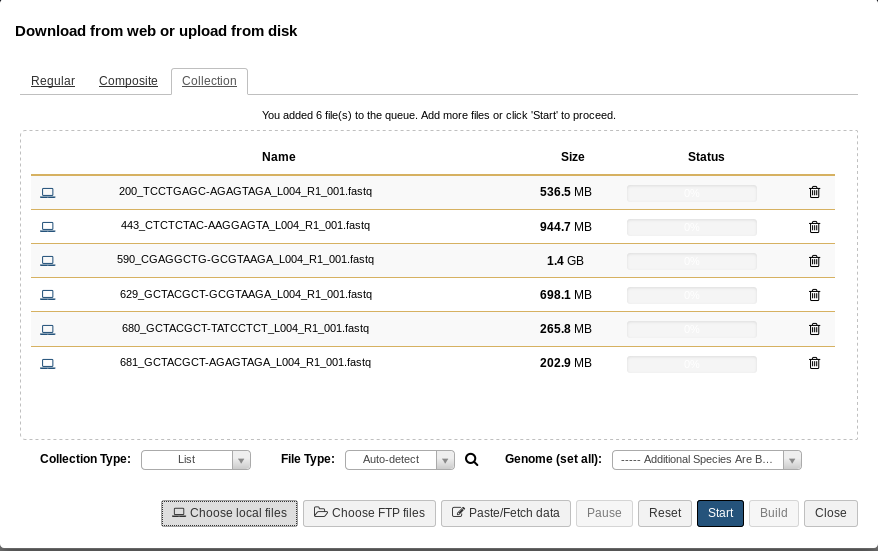
\includegraphics[scale=0.55]{images/SubidaDatasets.png}
      \caption{Interfaz de subida de los conjuntos de datos}
      \label{fig:SubidaDatasets}
    \end{center}
\end{figure}

En la vista de edición encontraremos un diagrama formado por las herramientas y uniones que indican las interacciones entre los ficheros de cada una de ellas. Al comienzo del proceso veremos dos cajas con el título <<Input dataset collection>>. Desde este paso se introducirán los datos de entrada al workflow en forma de una estructura denominada colección. Para ver cómo crear esa estructura saldremos un momento de la pestaña workflow, haciendo click en la opción <<Analyze data>> de la parte superior. A continuación, en el listado de categorías de herramientas que podemos ver en la parte izquierda, abriremos <<Get Data>> seguido de <<Upload File>>. Veremos como se despliega una ventana nueva en la que existen tres opciones de estructuras: <<regular>>, <<composite>> y <<collection>>. Deberemos seleccionar esta tercera opción y <<Choose local files>> para subir todos los ficheros del primer sentido de las secuencias. Es importante que los subamos en el mismo orden en el que lo vayamos a hacer con la colección de las secuencias en el sentido opuesto. Una vez seleccionados deberemos pulsar <<Start>> y, cuando las barras de progreso estén completas, <<build>>. Esto nos llevará a otra ventana en la que seleccionaremos el nombre de la colección con las lecturas en este sentido. Para finalizar, pulsaremos <<create list>>. Con este proceso tendremos una de las colecciones, y deberemos repetirlo para la colección con las lecturas en el sentido contrario. Cuando se hayan completado todos estos pasos, podremos volver a la vista de edición del workflow para seguir entendiendo su funcionamiento.


\begin{figure}
    \begin{center}
      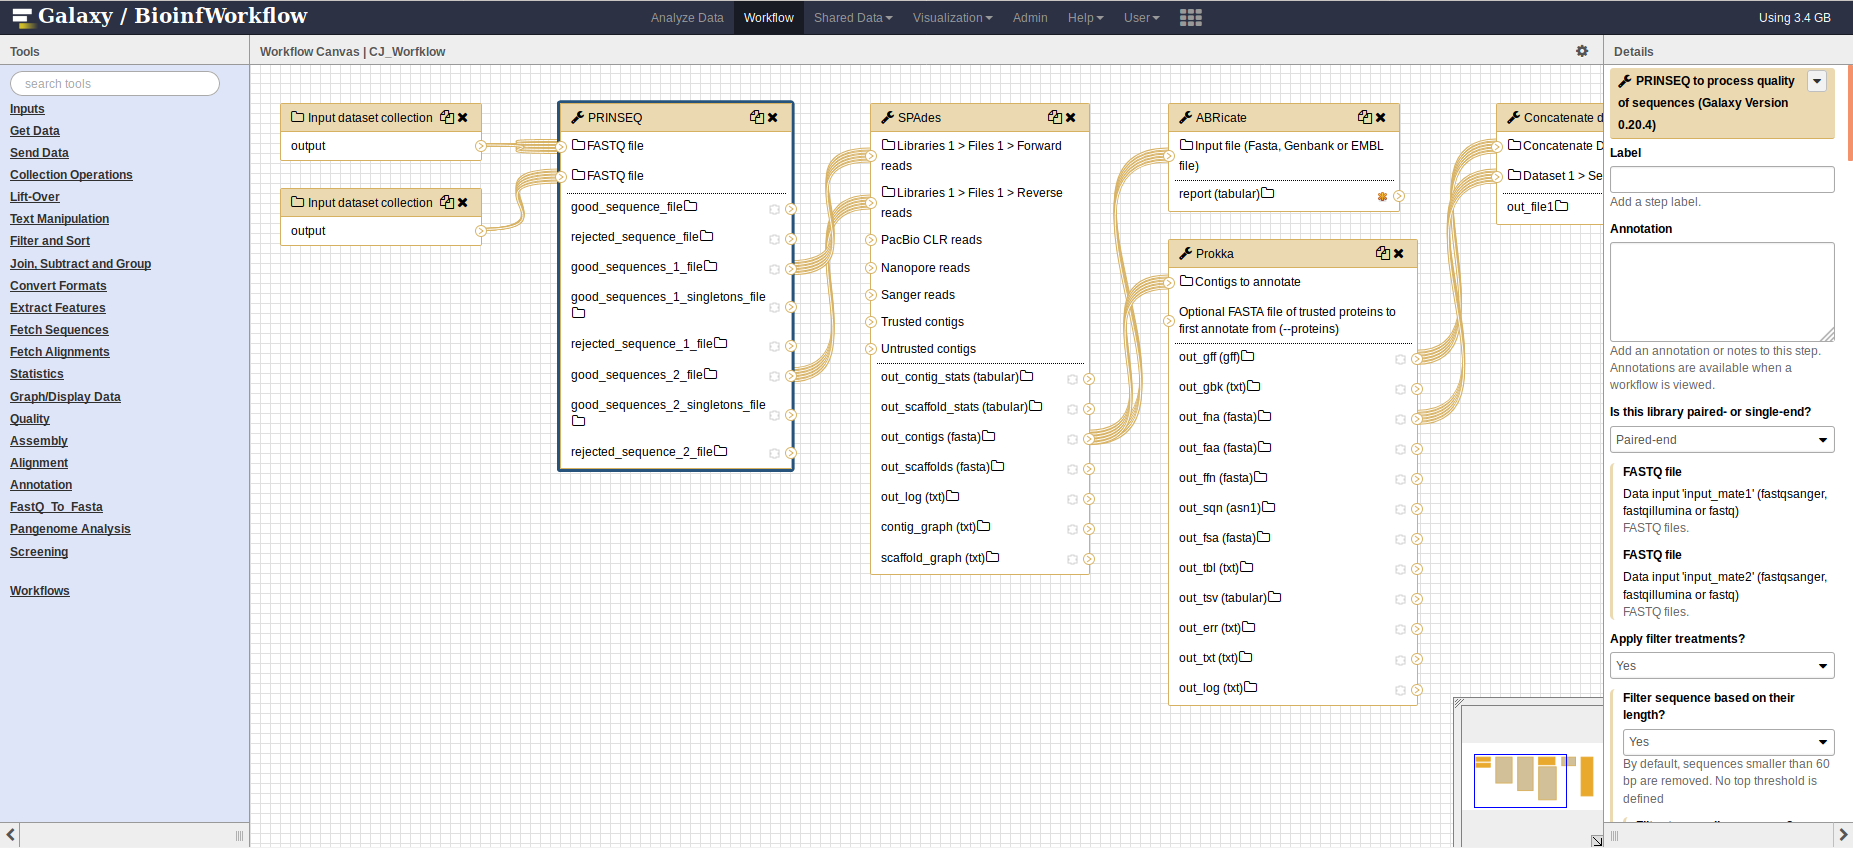
\includegraphics[scale=0.3]{images/InterfazWorkflowEdit.png}
      \caption{Interfaz de edición del workflow}
      \label{fig:WorkflowEdit}
    \end{center}
\end{figure}
Una vez visto el proceso de introducción de datos de entrada, encontramos las herramientas del workflow, cuyo funcionamiento se explica con más profundidad en el \autoref{chap:sistemadesarrollado}: <<Sistema, Diseño y Desarrollo>>. Para modificar los parámetros de cualquiera de las herramientas, podremos seleccionarla y veremos una serie de opciones en la parte derecha de la pantalla. Todos los parámetros modificados ya están guardados en el workflow, pero si se desea cambiar alguno de ellos, se podrá hacer desde esa interfaz. En caso de que se necesite añadir alguna herramienta extra, en el listado de la izquierda se encuentran ordenadas por categorías y con un clic serán añadidas, a falta de enlazar sus ficheros de entrada y de salida con las demás herramientas. Otro aspecto relevante a destacar es que, por defecto, en \textit{Galaxy} los datos se establecen como ocultos a no ser que se marquen con el asterisco que podemos ver a la derecha de los nombres de cada conjunto de datos de salida. Si hacemos clic en ese símbolo, los ficheros ya no aparecerán como ocultos y serán visibles en nuestro historial.

Los historiales son el sistema con el que \textit{Galaxy} ordena los conjuntos de datos del usuario. Desde la página de inicio <<Analyze Data>> podremos consultar el historial activo en este momento  en la parte derecha de la pantalla, pero este no tiene por qué ser el único que existe. Para consultar todos los historiales, desde la propia columna del historial activo, en la parte superior derecha, veremos tres símbolos con las opciones <<Refresh history>>, <<History options>> y <<View all histories>>. Desde esta última accederemos a una nueva pantalla en la que podremos consultar todos los historiales, Es posible que queramos ver conjuntos de datos ocultos de un historial, para ello, podremos activar la opción <<show hidden datasets>> situada debajo del nombre del historial.

Una vez comprendido el funcionamiento del workflow y los historiales, podremos ejecutar el workflow. Para ello, accederemos de nuevo a la pestaña <<Workflow> y desde el desplegable de <<CJ\_Workflow>> seleccionaremos la opción <<run>>. Esto nos situará en una nueva pantalla en la que, de nuevo, podremos modificar todos los parámetros de las herramientas del workflow. Sin embargo, es algo opcional en este momento. El punto principal es la introducción de los datos de entrada, que se seleccionarán desde dos desplegables (uno para cada sentido de las lecturas) en los apartados <<Input dataset collection>>. Si hemos creado las colecciones como se ha explicado previamente, estas aparecerán en el desplegable y solo tendremos que seleccionarlas. El paso siguiente, teniendo en cuenta que no queremos modificar ningún parámetro, será la ejecución del workflow usando el botón <<Run Workflow>> de la parte superior derecha.

A través del uso de los historiales, tendremos la opción de consultar el estado de las ejecuciones de cada una de las tareas del workflow. Teniendo en cuenta los pasos para consultar los historiales explicados anteriormente, podremos ver si una tarea se está ejecutando, en cola, pausada o si ha  causado algún error. Hay que tener en cuenta que es una ejecución computacionalmente muy costosa, por lo que puede llevar varias horas completarla. Por ello, es importante seguir el progreso a través del historial con el objetivo de asegurarnos de que no ha habido ningún error durante el proceso. Cuando todas las tareas se muestren en color verde, el workflow habrá completado su ejecución y podremos descargar los conjuntos de datos resultantes que nos interesen haciendo clic en ellos y seleccionando el icono con la opción <<download>>.

\begin{figure}
    \begin{center}
      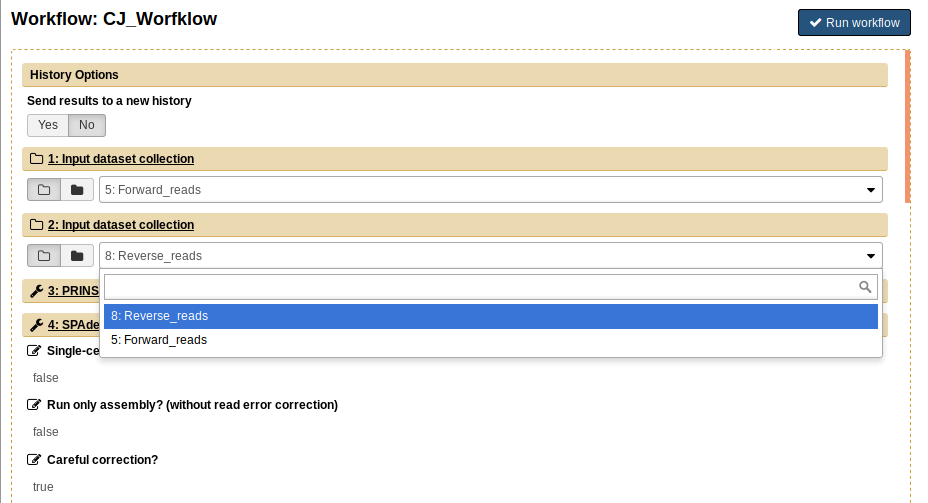
\includegraphics[scale=0.5]{images/RunInputs.png}
      \caption{Selección de las colecciones de entrada del workflow}
      \label{fig:RunInputs}
    \end{center}
\end{figure}

\subsection{Utilidad de ejecución simplificada}
Para facilitar el proceso explicado anteriormente, se ha desarrollado una utilidad que automatiza todos los pasos descritos. En el directorio <<exes>> del proyecto, encontramos un ejecutable llamado <<GalaxyWorkflow>>. Este programa es capaz de cargar los datos de entrada, crear las colecciones, ejecutar el workflow y descargar los resultados en una carpeta local sin necesidad de que el usuario interaccione con \textit{Galaxy}. 

En primer lugar, se requiere que la imagen Galaxy esté funcionando y podamos acceder a ella desde el navegador en la dirección <<http://localhost:8080/>>. Es conveniente realizar esta comprobación antes de ejecutar la aplicación. Si se desea, el usuario puede identificarse como administrador antes de comenzar, para poder consultar lo que está ocurriendo con \textit{Galaxy} mientras la utilidad está funcionando. Es importante dejar claro que interaccionará con dos nuevos historiales, así que para comprobar el funcionamiento, si es que se desea, se deberá hacer desde la vista de todos los historiales.

El proceso para ejecutarlo es muy sencillo, solamente deberemos abrir la terminal de Ubuntu y situarnos en el directorio <<exes>> del proyecto. Una vez ahí, veremos que existen dos carpetas <<Forward>> y <<Reverse>>. En ellas deberemos introducir los ficheros <<.fastq>> de las lecturas que deseamos analizar. Los ficheros de cada sentido de lectura deben dividirse en las dos carpetas. Es necesario que ambas tengan el mismo número de ficheros y muy recomendable que los nombres de los dos sentidos de una lectura comiencen por el mismo identificador único. Por ejemplo, dos nombres de una pareja podrían ser  <<lectura\textbf{1}\_forward>> y <<lectura\textbf{1}\_reverse>>. Cuando contemos con todos los ficheros situados en los directorios corresponientes, escribiremos el siguiente comando.
\begin{lstlisting}[language=bash]
    $ ./GalaxyWorkflow
\end{lstlisting}
Con ello, comenzará la ejecución y cada minuto recibiremos una actualización del estado de las tareas en marcha, pudiendo comprobar si ha habido algún error y ser capaz de detener la ejecución desde \textit{Docker}. Si esto sucediera, la manera más fácil sería detener la imagen \textit{Galaxy} con el comando:
\begin{lstlisting}[language=bash]
    $ ./stop.sh
\end{lstlisting}
O, incluso, resetear la imagen de cero para eliminar todos los ficheros que ya no nos interesan, con la combinación de comandos
\begin{lstlisting}[language=bash]
    $ ./stop.sh
    $ ./remove.sh
    $ ./run.sh
\end{lstlisting}
Normalmente, esto no será necesario y, tras varias horas de ejecución, obtendremos los resultados en un directorio <<ResultsHistory[+timestamp]>> en el que serán ordenados en carpetas dependiendo de la herramienta de la que provengan.

\subsection{Tratamiento de datos obtenidos}
Con la utilidad del apartado anterior, obtenemos un gran número de ficheros independientes. El objetivo de esta herramienta es agrupar los resultados de \textit{ABRicate} y \textit{Roary} en un solo documento <<.xls>> que podamos abrir como una hoja de cálculo. Para ello, deberemos situarnos de nuevo en el directorio <<exes>>. Nuestros datos de entrada estarán situados en una carpeta con un nombre que comience por <<Results>> y que contenga varias subcarpetas, cada una con el nombre de la herramienta de origen de los ficheros que contiene. Por ejemplo, dos carpetas: <<roary>> y <<abricate>> con los ficheros resultantes de cada una en su interior. Una vez tengamos esta estructura (que por defecto se cumple si se utiliza la herramienta de ejecución automática del workflow) podremos abrir la terminal en el directorio <<exes>> e introducir el comando
\begin{lstlisting}[language=bash]
    $ ./OutputToXls
\end{lstlisting}
Esto generará un fichero con el mismo nombre que la carpeta que hemos indicado anteriormente pero con extensión <<.xls>> en el que cada hoja del documento corresponderá a una de las herramientas.
\newpage \thispagestyle{empty} % Página vacía 

\chapter{Manual del programador}
\label{Anexo:codigosMatlab}


\newpage \thispagestyle{empty} % Página vacía 


%Hoja final en blanco
\newpage \thispagestyle{empty} % Página vacía

\end{document}
